For the sake of completeness, we recall here some standard definitions and properties about entanglement entropy. We also take the opportunity to set some notations and conventions that will be used throughout this report. This review is mainly based on chapter 2 and 3 of Matthew Headrick's lecture \cite{entropy}.

\section{Von Neumann entropy}

One of the ultimate differences between classical and quantum mechanics is that in quantum mechanics one can not separate between the notion of state of a system and the knowledge we have on the state of the system. In quantum mechanics, we encode this information in an operator named \textbf{density matrix} obeying the following:
\begin{align}\label{properties of rho}
    \rho^\dagger = \rho,         &&           \rho \geq 0,          &&        \text{Tr}\rho=1.
\end{align}

We distinguish between two types of states. A state is called \textbf{pure} if it can be written as a one dimensional projector,
\begin{equation}\label{pure state}
    \rho = \ket{\psi}\bra{\psi}.
\end{equation}
In this case, $\rho$ cannot be written as a linear combination of other states. The expectation value of observables simply takes the form $\Braket{A}=\bra{\psi}A\ket{\psi}$.

The rest of the states are \textbf{mixed}. These are statistical ensembles of pure states. One way to distinguish between pure and mixed states is by computing $\text{Tr}\rho^2$. This trace is obviously equal to 1 in the case of (\ref{pure state}) and is less than 1 for mixed states. Geometrically, pure states are represented as vectors on the surface of the Bloch-Sphere whilst mixed states are represented with vectors inside the sphere.

It is important to note that, using (\ref{properties of rho}), the density matrix can be diagonalized,
\begin{equation}
    \rho = \sum_a p_a\ket{a}\bra{a}
\end{equation}
where $p_a$ is a probability distribution.

The entropy of the state $\rho$ comes natural from the \textit{Shannon entropy} in the classical case \cite{bengtsson_zyczkowski_2006},
\begin{equation}\label{Von Neumann}
    S\left(\rho\right):=S\left(\Vec{p}\right)=-\text{Tr}\rho\ln \rho = \braket{-\ln\rho}_\rho.
\end{equation}
This is known as the \textbf{Von Neumann entropy}. It is non negative and vanishes if and only if $\rho$ is a pure state. It is also invariant under unitary transformation, i.e unitary transformations are reversible.

Things get more interesting when we consider a joint system $AB$. The Hilbert space of the joint system is
\begin{equation}
    \mathcal{H}_{AB}\cong \mathcal{H}_A\otimes\mathcal{H}_B    
\end{equation}
where $\cong$ means isomorphic (same structure). We can always find the state of the subsystem $A$ by taking the trace over $B$,
\begin{equation}
    \rho_A := \text{Tr}_B\rho_{AB}.
\end{equation}
This is the \textbf{reduced density matrix}. The Von Neumann entropy (\ref{Von Neumann}) is extensive and subadditive,
\begin{equation}
    S\left(AB\right) \leq S\left(A\right) + S\left(B\right)
\end{equation}

There are two other important inequalities that are obeyed by the entropies of subsystems. The first one is the \textbf{Araki-Lieb} inequality,
\begin{equation}\label{Araki-Lieb}
    S\left(AB\right) \geq \left|S\left(A\right) - S\left(B\right)\right|
\end{equation}
and the second called the \textbf{strong subadditivity},
\begin{equation}\label{weak monotonicity}
    S\left(AB\right) + S\left(BC\right) \geq S\left(A\right) + S\left(C\right).
\end{equation}

An important result of (\ref{Araki-Lieb}) is that $S\left(A\right) = S\left(B\right)$ if $AB$ is a pure state.

\section{Entanglement}
There has been many works in the area of quantum entanglement measurements. Entanglement entropy is the main measurement tool to quantify entanglement, especially in the case of pure states. But there are many considerable different ways to quantify the amount of entanglement like the entanglement cost, distillable entanglement or entanglement of formation \cite{Virmani}.

Entanglement entropy  is a measure of how quantum information is spatially organised in a quantum state. We distinguish between two cases: $AB$ pure and $AB$ mixed.

\subsection{Pure state}
A pure state (\ref{pure state}) that cannot be factorized into the product of two,
\begin{equation}\label{factorized state}
    \ket{\psi} = \ket{\psi'}_A\otime\ket{\psi''}_B
\end{equation}
is \textbf{entangled}. One can consider the famous example of a \textbf{Bell pair} \cite{Bell}, a qubit bipartite system $AB$ in the pure state
\begin{equation}\label{Bell pair}
    \ket{\psi}=\frac{1}{\sqrt{2}}\left(\ket{0}_A\otimes\ket{1}_B+ \ket{1}_A\otimes\ket{0}_B\right).
\end{equation}
We can verify the entanglement of $A$ and $B$ by computing their corresponding entanglement entropy through their reduced density matrix (\ref{psiA}), see Appendix \ref{appendix A}. If it is different than zero then the subsystems are mixed which indicates that they are entangled.
\begin{equation}\label{psiA}
    \rho_A := \text{Tr}_B\rho = \frac{1}{2}\left(\ket{0}_A\bra{0}+\ket{1}_A\bra{1}\right)
\end{equation}
There is a connection between entanglement and factorization in the case of a pure state. The state $\rho_{AB}$ can be factorized if and only if $\rho_A$ is pure, which is true if and only if $\rho_B$ is pure. An important fact to mention is that if we start with an unentangled state $\rho_{AB}$, no combination of \textit{local operations} on $A$ and $B$ and no \textit{classical communication} between $A$ and $B$ (\textbf{LOCC})  will result in a pure entangled state. In other words, if the two subsystems $A$ and $B$ are to be entangled, it requires the action of a third party.

Entropies are bounded by the log of the dimension of their Hilbert space. This is obvious following the definition (\ref{Von Neumann}). In the limit of a large Hilbert space, this bound becomes saturated and we have,
\begin{equation}
    S\left(A\right) = \min \left\{ \ln\dim\mathcal{H}_A,\ln\dim\mathcal{H}_B\right\} + \mathcal{O}(1).
\end{equation}

As an example, if $AB$ is a system of large number of spins where a touch $x$ is part of $A$ and the rest belongs to $B$, then the entanglement entropy follows what we call a \textbf{Page curve} as a function of $x$, fig. \ref{page curve}. At the start, the Page curve was a model used in black hole physics, being considered in pure state at $t_0$, to understand its evaporation process. The subsystem $A$ containing the black hole becomes entangled with outgoing Hawking radiations $B$ throughout the evaporation process. The Black hole's EE is supposed to follow a Page curve.

\begin{figure}
    \centering
    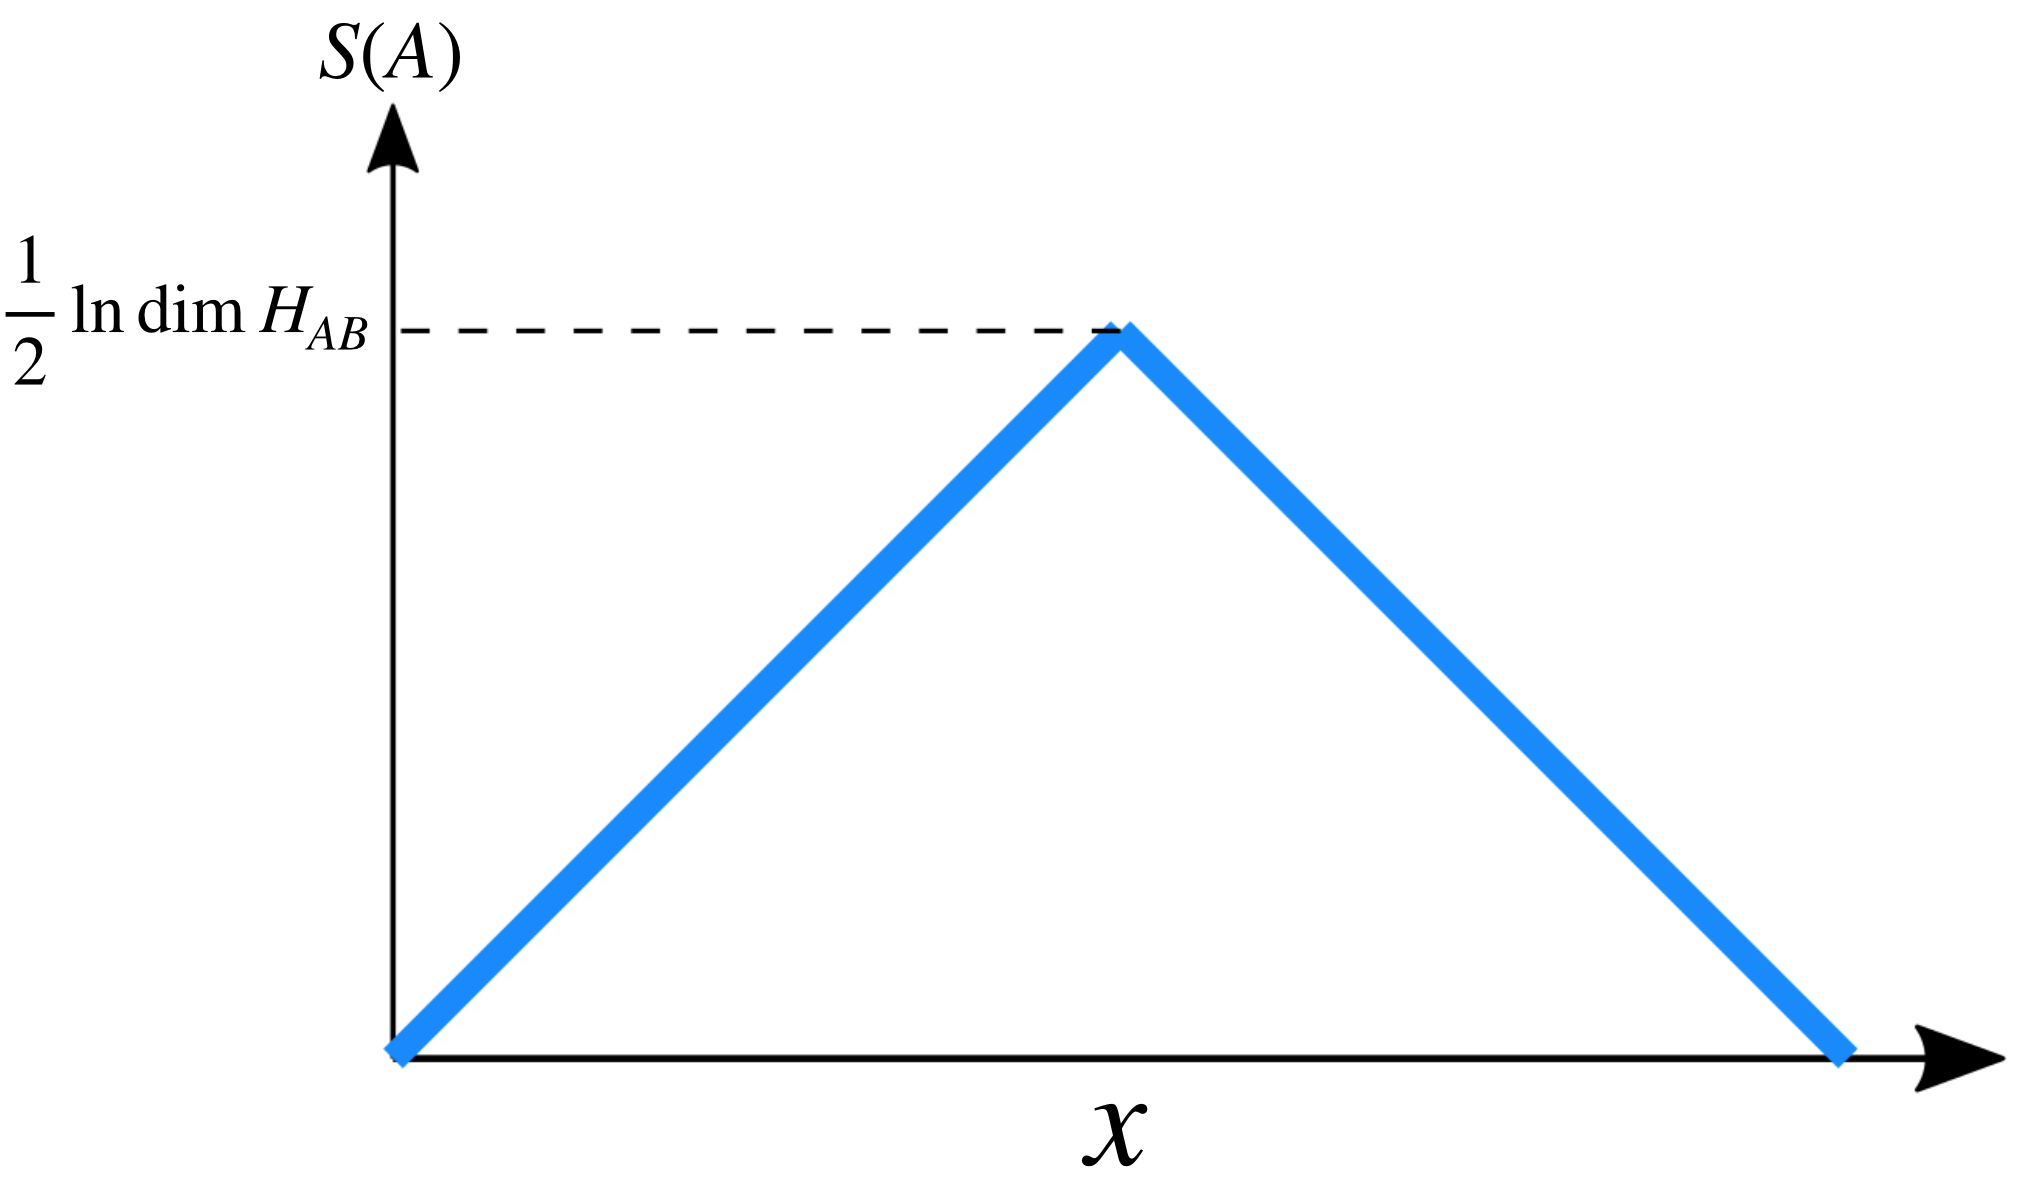
\includegraphics[width=0.65\textwidth]{figures/page_curve.png}
    \caption{The EE $S(A)$ of a subset $A$ of a larger system $AB$ in a pure state. $AB$ is a system of large spins where a fraction $x$ of them belongs to $A$. The EE follows a Page curve.}
    \label{page curve}
\end{figure}

\subsection{Mixed state}
In the case of mixed states, the results mentioned in the previous subsection are almost lost. We say that a state is not entangled if it is separable (classically correlated), i.e
\begin{equation}
    \rho = \sum_ip_i{\rho^i}_A\otimes{\rho^i}_B.
\end{equation}

Detecting entanglement and its type (classical or quantum) turns out to be a very (NP-)hard problem\cite{gharibian2009strong}. One way to detect this entanglement is to compute the sign of the \textbf{conditional entropy}
\begin{equation}\label{conditional entropy}
    H\left(A|B\right):=S\left(AB\right)-S\left(B\right)
\end{equation}
which is positive in the classical case and for separable states. This condition is sometimes violated in the presence of entanglement, like in the case of an entangled pure state,
\begin{equation}\label{negative H(A|B)}
    H\left(A|B\right) = -S\left(B\right)\leq 0.
\end{equation}

\subsection{Monogamy of entanglement}

One last feature we mention on entanglement is the property of monogamy. This comes from the strong subadditivity (\ref{weak monotonicity}) which can be rewritten as (see Appendix \ref{appendix A}),
\begin{equation}\label{SSA}
     H\left(B|A\right) + H\left(B|C\right)\geq 0.
\end{equation}
This shows that at most, one of the pairs $AB$ or $CB$ can be entangled.

In the case of black hole evaporation, this monogamy represents an issue. Consider a black hole at a time $t$ where more than half of the radiation has been emitted. The next outgoing Hawking quanta "$B$" will be entangled with those previously emitted "$A$" while at the same time it is entangled with ingoing particles "$C$". Many explanations have been suggested to solve this paradox. One proposition by AMPS\cite{Almheiri_2013} suggested a firewall at the horizon shielding the falling observers from entering the black hole. This proposal was criticized as it violates Einstein's equivalence principal. Maldacena and Susskind \cite{Maldacena_2013} proposed in ER=EPR that outgoing and ingoing Hawking quanta are connected through a wormhole and as a result should not be considered as independent systems.

\section{Thermofield double}

Mixed states can always be considered to be part of a larger system $\Tilde{H} = H\otimes K$ which is in a pure state. To get back the original system, we can trace over the complement system $K$. This method goes under the name of purification \cite{Kleinmann_2006}.

One way to perform this purification is through the \textbf{thermofield double}.  In this method, the pure state is created by doubling the original system $A$. Consider for example a \textbf{Gibbs state}
\begin{equation}\label{Gibbs state}
    \rho_A = \frac{1}{Z}\sum_a e^{-\beta E_a}\ket{a}_A\bra{a}.
\end{equation}
We choose $K$ to be a copy of the original system $\mathcal{H}_A$. The thermofield double state is
\begin{equation}\label{thermofield double}
    \ket{\phi} = \frac{1}{\sqrt{Z}}\sum_a e^{-\beta E_a/2}\ket{a}_A\otimes\ket{a}_B.
\end{equation}

If the purification was made by a different system, the resulting state $\ket{\chi}$ is related to the thermofield double by a unitary transformation,
\begin{equation}
    \ket{\chi} = I_A\otimes U_B \ket{\phi}.    
\end{equation}
This is known as the Schrödinger–HJW theorem, \cite{schrodinger_1936}.

The thermofield double state can be written in terms of an Euclidean path integral on a semicircle of length $\beta/2$. This can be seen if we write the operator $e^{-\beta H}$ as an Euclidean path integral over an interval of length $\beta$. It's matrix element is a path integral with boundary conditions and can be represented as
\begin{equation}\label{l3iba}
    \bra{x_0}e^{-\beta H}\ket{x_1} = \ctikz{\draw (0.967,0.255) arc (10:350:1);\node at (0.967,0.255) [circle,fill=red,inner sep=1.5pt]{}; \node at (0.96,-0.150) [circle,fill=red,inner sep=1.5pt]{};
    \draw node at (1.3,-0.2){$x_0$};\draw node at (1.3,0.2){$x_1$};},
\end{equation}
where the circle is of length $\beta$. The component of the thermofield double state in $\ket{x_a}\otimes\ket{x_b}$ is
\begin{equation}
    \left(\bra{x_a}\otimes\bra{x_b}\right)\ket{\phi} = \frac1{\sqrt{Z}} \times \ctikz{\draw (-1,0) arc (180:360:1);\node at (-1,0) [circle,fill=red,inner sep=1.5pt]{}; \node at (1,0) [circle,fill=red,inner sep=1.5pt]{};
    \draw node at (-1.3,0){$x_0$};\draw node at (1.3,0){$x_1$};}.
\end{equation}
where the circle is of length $\beta/2$. One can check that tracing (\ref{thermofield double}) gives back exactly the original Gibbs state (\ref{Gibbs state}). This can also be checked in the path integral formulation as done in appendix \ref{appendix A}. This shows how thermal states are originated from entanglement in a larger system.

\section{Fine-grained vs Coarse-grained entropy}

There are two notions of entropy that will be of use in the following chapters: fine-grained and coarse-grained entropy.

The fine-grained entropy is the von Neumann entropy (\ref{Von Neumann}) we discussed above. As we mentioned earlier, it quantifies our ignorance on the system and most importantly it is invariant under unitary evolution $\rho\rightarrow U\rho U^{-1}$.

The coarse-grained entropy is defined as follows. Having a density matrix $\rho$ that describes our system, we consider all possible states $\Tilde{\rho}$ such that the subset of observables $A_i$ that we are considering is unchanged, $\text{Tr}[\Tilde{\rho}A_i]=\text{Tr}[\rho A_i]$. Then we maximize the von Neumann entropy over $\Tilde{\rho}$. This definition increases with unitary time evolution and therefore obeys the second law of thermodynamics. 

One important point to mention, though obvious, is that the fine-grained entropy is always smaller than the coarse-grained entropy by definition,
\begin{equation}
    S_{vN}\leq S_{\text{coarse}}.    
\end{equation}

A simple example of the coarse-grained entropy is the thermodynamic entropy, where the observables subset contains energy and volume.

\section{Entanglement entropy in Field theories}

One can consider field theories to be the limit of lattice systems where the lattice spacing goes to zero $a\rightarrow0$ to obtain a continuous spacial region as shown in fig. \ref{lattice system}. The Hilbert space of such a system is the direct product of local Hilbert spaces,
\begin{equation}
    \mathcal{H} = \otimes_{x}\mathcal{H}_x.
\end{equation}

In relativistic quantum field theory, this spacial region can be replaced by a Cauchy slice $\sigma$. Since observables on Cauchy slices in different points commute, a region $A\in\sigma$ comes with a factorization of the Hilbert space as
\begin{equation}
    \mathcal{H} = \mathcal{H}_{A} \otimes \mathcal{H}_{A^c},
\end{equation}
up to some technicalities in the entanglement surface. This spacial region has the same entropy as any other region that shares with $A$ the same causal domain $D(A)$\footnote{The caudal domain $D(A)$ of a region $A$ is the group of all the points that are only causally related to $A$.},
\begin{equation}
    D(A) = D(A') \implies S(A) = S(A').
\end{equation}

\begin{figure}
    \centering
    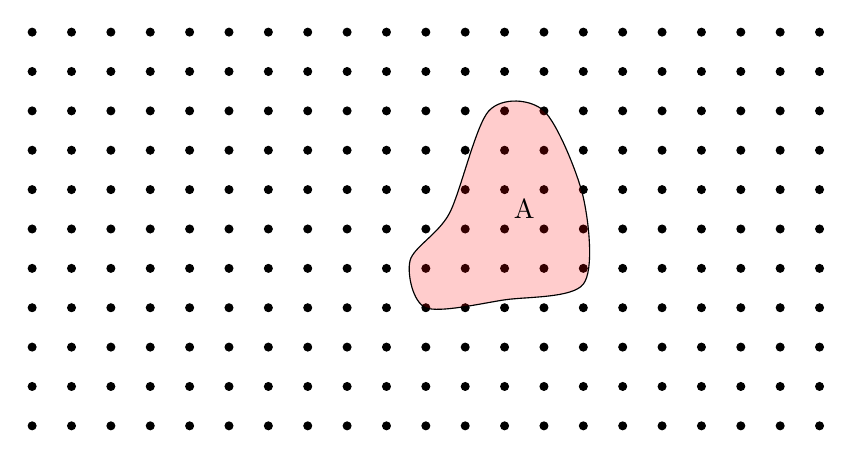
\begin{tikzpicture}
        [%%%%%%%%%%%%%%%%%%%%%%%%%%%%%%
            dot/.style={circle,draw=black, fill,inner sep=1pt},
        ]%%%%%%%%%%%%%%%%%%%%%%%%%%%%%%
        
        \foreach \x in {0,...,20}{
            \foreach \y in {0,...,10}{
                \node[dot] at (\x/2,\y/2){ };
            }
        }

        \draw[fill=red,opacity=0.2] plot [smooth cycle] coordinates {(5,1.5) (6,1.6) (7,1.8) (7,2.9) (6.5,4) (5.8,4) (5.3,2.7) (4.8,2.1) } node at (6,2.5){};
        \draw plot [smooth cycle] coordinates {(5,1.5) (6,1.6) (7,1.8) (7,2.9) (6.5,4) (5.8,4) (5.3,2.7) (4.8,2.1) } node at (6.25,2.75){A};
    \end{tikzpicture}
    \caption{Region $A$ of a lattice system with lattice spacing $a$.}
    \label{lattice system}
\end{figure}

Entanglement entropies in field theories are usually computed using path integrals and the replica trick. This method consists of considering $n$ replicas of the original system and compute,
\begin{equation}
    Z_n=\text{Tr}\rho^n.
\end{equation}
The von Newman entropy is then found by deriving $Z_n$ with respect to $n$ and setting $n=1$. These methods are usually complicated to compute. However, theories admitting holographic description (in the sense of AdS/CFT correspondence), entanglement entropies can be found through a simple computation of minimal surfaces. This will be the subject of the next chapter. 
